% Provenance (never printed): see sources/outline_sources.md (Year 2: palaeogeography through
% the Phanerozoic; sea level; orogenies; mass extinctions and their Earth causes). Maps from the
% plate model of Merdith and others (2021) through the GPlates Web Service; sea level from the
% Miller and others (2005) NOAA study (Haq and others 1987; Kominz and others 2008); flooding and
% the Pitman model after Tasistro-Hart and Macdonald (2023); the big five after Marshall (2023)
% and Kaiho (2022); oceanic anoxic events after Rigo and others (2024) and Walker-Trivett and
% others (2024); CAMP carbon dioxide after Capriolo and others (2020); Chicxulub after
% Pickersgill and others (2026) and Collins and others (2020). Curves and numbers from
% figdata/bachelor-2/phanerozoic.py; exercise and problem values in the Book 4 scratch
% calculator calc/ch19.py.
\chapter{Bumi Fanerozoikum}\label{ch:b2:phanerozoic-earth}

Di Kansas bagian barat, di tengah Amerika Utara, tiang-tiang kapur putih menjulang dari
padang rumput. Kapur itu adalah lumpur dasar laut: sekitar 80 juta tahun yang lalu sebuah laut
dangkal membentang dari utara ke selatan melintasi tengah Amerika Utara, dan cangkang
alga yang melayang mengendap di dasarnya dengan laju beberapa perseratus milimeter per tahun. Lima kali dalam
540 juta tahun terakhir, sebagian besar spesies yang hidup di laut seperti itu lenyap dalam
sekejap waktu geologi. Kedua kisah itu adalah kisah Bumi sendiri: benua-benua bergerak dan laut naik dan turun di atas
benua-benua itu, dan sedikitnya tiga dari lima kepunahan besar bertepatan dengan curahan lava dari dalam
planet. Bab ini mengikuti Fanerozoikum melalui peta-petanya, muka lautnya, sabuk-sabuk
pegunungannya, dan krisis-krisisnya, dan menyatakan dua di antaranya dalam angka: seberapa cepat punggungan menaikkan laut, dan seberapa luas
daratan yang ditenggelamkan oleh laut yang lebih tinggi.
% ledger: kgs:monument-rocks, kgs:chalk, ics:base.Phanerozoic, kaiho22:table, cr03:table

\begin{recall}
\textbf{Dari volume-volume sekolah}: tektonik lempeng dan Pangea; fosil dan skala waktu
geologi; transgresi yang dibaca pada sebuah tebing. \textbf{Dari volume Tahun 1}: hukum kedalaman--umur
dasar samudra; kurva hipsometrik; isostasi; eustasi dan muka laut relatif; provinsi beku
besar; kepunahan massal sebagai penanda stratigrafi, iridium pada batas K--Pg, dan
penentuan umur krisis akhir Perm; jenjang dan GSSP. \textbf{Dari bab-bab sebelumnya}: \omterm{def:b2:alpine-orogen:orogen}{orogen}
(\cref{ch:b2:alpine-orogen,ch:b2:himalaya-andes}); \omterm{def:b2:wilson-cycle:wilson}{siklus Wilson} dan \omterm{def:b2:wilson-cycle:supercontinent}{superbenua}
(\cref{ch:b2:wilson-cycle}); \omterm{def:b2:basins-compared:backstripping}{pengupasan balik} (\cref{ch:b2:basins-compared}); bola salju
Kriogenian (\cref{ch:b2:precambrian-earth}). Kepunahan dan sejarah kehidupan termasuk buku-buku
biologi; volume Tahun~3 membahas paleomagnetisme dan stratigrafi sekuen.
\end{recall}

\section{Peta-peta dunia yang bergerak}\label{sec:b2:phanerozoic-earth:maps}

Sebuah batuan jarang berada di tempat ia terbentuk. Batu bara, batu pasir gurun, terumbu: masing-masing diendapkan pada
suatu lintang dan sejak itu terbawa oleh lempengnya. Sebelum iklim atau kehidupan suatu masa
lampau dapat dibaca dari batuan seperti itu, batuan itu harus dikembalikan ke tempatnya semula.

\begin{definition}[Paleogeografi; peta paleogeografi]\label{def:b2:phanerozoic-earth:palaeogeography}
Yang disebut \emph{paleogeografi}\index{paleogeografi} adalah rekonstruksi geografi suatu masa
lampau: kedudukan benua dan samudra, serta garis pantai, sabuk pegunungan, dan
lautnya. Sebuah \emph{peta paleogeografi}\index{peta paleogeografi} menunjukkan geografi itu pada satu
waktu, pada kisi lintang dan bujur waktu itu.
\end{definition}

Empat jenis bukti masuk ke dalam peta seperti itu. Magnetisasi batuan memberikan lintang tempat
batuan itu terbentuk, pokok bahasan paleomagnetisme dalam volume Tahun~3; tetapi medan Bumi
simetris terhadap sumbunya, sehingga medan itu tidak mengatakan apa pun tentang bujur. Dasar samudra merekam gerak
lempeng secara langsung, melalui pita-pita magnetiknya dan umurnya, tetapi hanya sampai
dasar samudra tertua yang masih tersisa, sekitar 190 juta tahun: semua yang lebih tua telah tersubduksi. Sebelum itu,
kecocokan bentuk benua-benua, sutur dan \omterm{def:b2:alpine-orogen:orogen}{orogen} tempat samudra menutup, serta fosil dan
sedimen yang membuka rahasia suatu iklim --- terumbu dan evaporit di daerah tropis, endapan glasial dekat
kutub --- melengkapi gambarannya. Model lempeng mengumpulkan batasan-batasan ini dan memutar setiap lempeng kembali dalam
waktu; rekonstruksi juga harus memperhitungkan rotasi lambat seluruh Bumi padat terhadap
sumbu putarnya, yang disebut pengembaraan kutub sejati.
% ledger: vh26:palaeogeography, gws:merdith-frame, data:b2-seafloor-age, merdith21:model

\begin{omfigure}
\centering
% figdata/bachelor-2/phanerozoic.py parts map-<t>, cities-<t>, grat (Mollweide, x and y in Earth radii)
\begin{tikzpicture}
\begin{groupplot}[group style={group size=2 by 3, horizontal sep=0.35cm, vertical sep=0.55cm},
  width=0.53\linewidth, axis equal image, hide axis, clip=false,
  xmin=-2.85, xmax=2.85, ymin=-1.43, ymax=1.43,
  title style={font=\small, yshift=-1.5ex}]
\pgfplotsinvokeforeach{500,300,200,100,50,0}{
\nextgroupplot[title={#1~\unit{Ma}}]
\fill[omSea] (axis cs:0,0) ellipse [x radius=2.8284, y radius=1.4142];
\addplot[fill=omLithAlluv!85!black, draw=none] table[x=x, y=y]
  {figdata/out/bachelor-2-phanerozoic-map-#1.dat};
\addplot[black!35, line width=0.2pt] table[x=x, y=y] {figdata/out/bachelor-2-phanerozoic-grat.dat};
\draw[black!70, line width=0.4pt] (axis cs:0,0) ellipse [x radius=2.8284, y radius=1.4142];
\addplot[only marks, mark=*, mark size=1.3pt, red!75!black, point meta=explicit symbolic,
  nodes near coords, nodes near coords style={font=\tiny\bfseries, anchor=south west,
  inner sep=0.5pt, text=red!60!black}]
  table[x=x, y=y, meta=tag] {figdata/out/bachelor-2-phanerozoic-cities-#1.dat};
}
\end{groupplot}
\end{tikzpicture}
\par\smallskip{\small Garis pantai masa kini yang dibawa kembali ke enam waktu dalam model lempeng
Merdith dan kawan-kawan (2021), direkonstruksi oleh GPlates Web Service, dalam proyeksi Mollweide
luas-sama; garis lintang setiap \ang{30}, garis bujur setiap \ang{60}. Titik-titik merah mengikuti empat
kota: Paris (P), New York (N), Sydney (S), dan Cape Town (C); pada \qty{500}{Ma} kerak
Sydney belum ada dalam model. Bentuk-bentuk itu adalah garis pantai masa kini yang dipindahkan, bukan garis pantai
masa itu, dan dalam kerangka paleomagnetik ini bujurnya sembarang.}
\end{omfigure}
% ledger: data:b4-palaeocoast, data:b4-palaeopos, geonames4:cities, gws:merdith-frame, merdith21:model

Keenam peta di atas adalah Fanerozoikum secara ringkas. Pada \qty{500}{Ma} benua-benua selatan membentuk
satu massa, Gondwana, yang sebagian besar dekat Kutub Selatan, dengan kerak Paris pada \ang{61}~LS di
tepinya. Pada \qty{300}{Ma} benua-benua telah bergabung menjadi Pangea, yang terhimpun sejak sekitar
\qty{325}{Ma} dan terpecah sejak sekitar \qty{200}{Ma}: Paris dan New York terletak di khatulistiwa, Cape
Town dan Sydney dekat \ang{60}~LS. Pada \qty{200}{Ma} \omterm{def:b2:wilson-cycle:supercontinent}{superbenua} itu lengkap, satu daratan
yang membentang dari lintang tinggi utara sampai lintang tinggi selatan; pada \qty{100}{Ma} Samudra Atlantik dan Samudra Hindia telah membuka, dan pada
\qty{50}{Ma} peta itu hampir sama dengan peta kini, dengan Australia masih dekat Antartika.
% ledger: data:b4-palaeopos, nance22:supercontinents

\begin{example}[Paris bergeser ke utara]\label{ex:b2:phanerozoic-earth:paris}
Dalam model itu, Paris terletak pada \ang{5.1}~LU \qty{300}{Ma} yang lalu; kini ia terletak pada \ang{48.9}~LU.
Lintangnya bertambah \ang{43.8}, yaitu $43.8 \times 111.2 = \qty{4871}{km}$ sepanjang meridian
($\qty{111.2}{km}$ per derajat pada bola berjari-jari \qty{6371}{km}), dengan laju rata-rata
$4871/300 = \qty{16}{km}$ per juta tahun, atau \qty{1.6}{cm} per tahun. Ini hanya komponen gerak
ke utara: kerangka paleomagnetik membiarkan bujur bebas, sehingga jarak sebenarnya yang
ditempuh sedikitnya sebesar ini.
\end{example}
% ledger: data:b4-palaeopos, geonames4:cities, earth:Rmean, gws:merdith-frame
% values: calc/ch19.py (43.8 deg, 4870.6 km, 16.2 km/Myr)

\section{Muka laut sepanjang Fanerozoikum}\label{sec:b2:phanerozoic-earth:sealevel}

\subsection*{Laut di atas benua}

Selama sebagian besar Fanerozoikum, jauh lebih banyak bagian benua yang berada di bawah laut daripada kini. Batuan
laut Amerika Utara merekam beberapa banjir di pedalaman benua itu, yang pertama di antaranya
transgresi Kambrium yang menutup Ketidakselarasan Besar; pada Kapur Akhir, dari
sekitar 120 sampai \qty{80}{Ma}, sedimen laut terakumulasi di seluruh Western Interior, di tengah
benua (foto di bawah).
% ledger: th23:flooding, th23:wib

\begin{omfigure}
\centering
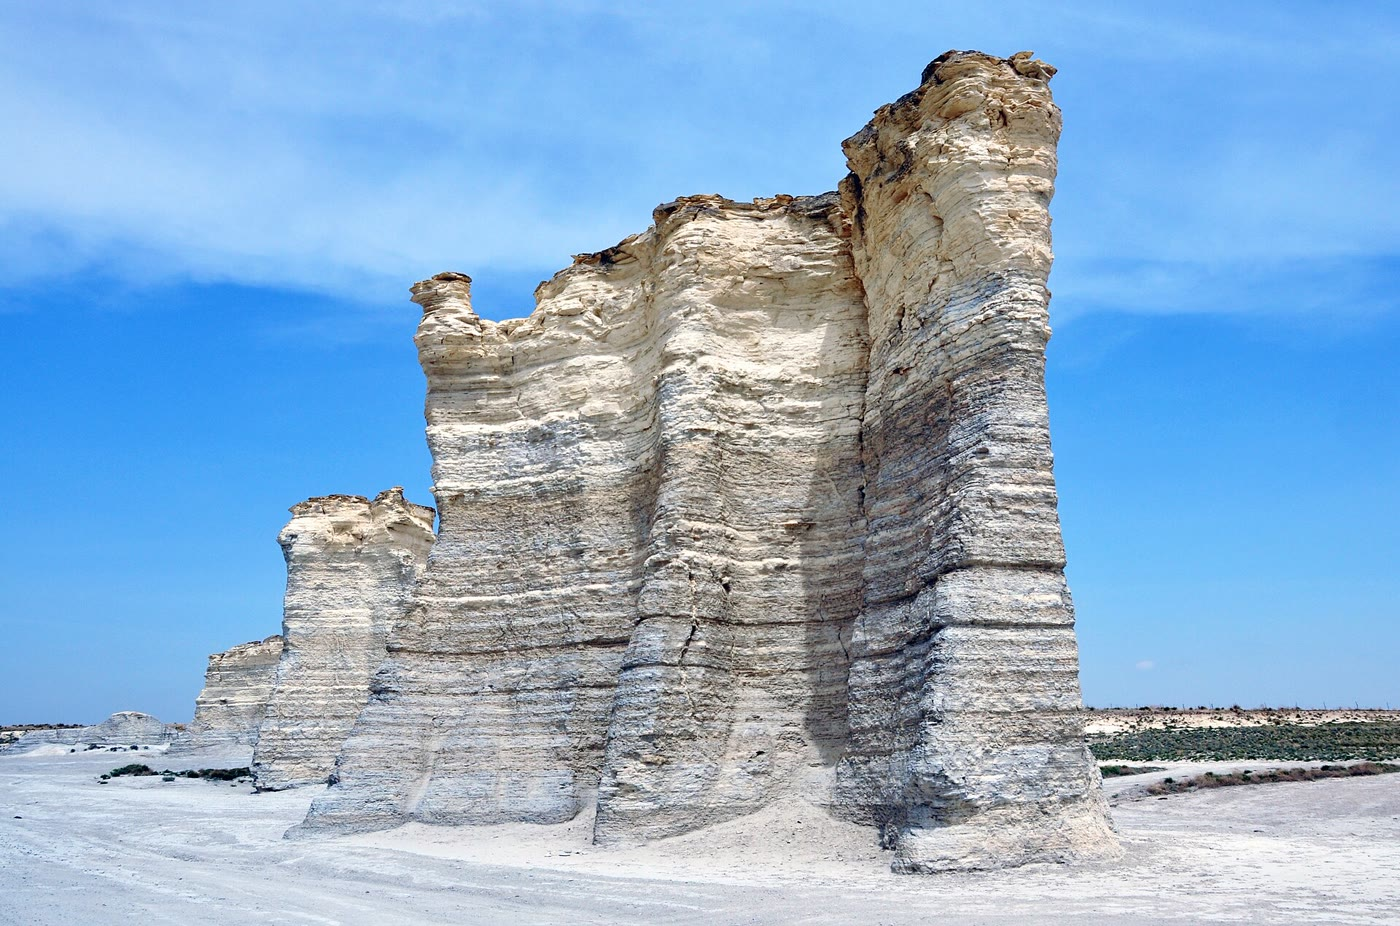
\includegraphics[width=0.66\linewidth]{images/book4/b2-19-monument-rocks.jpg}
\par\smallskip{\small Monument Rocks, Kansas bagian barat: tiang-tiang kapur, lumpur sebuah laut pedalaman
Kapur yang berumur sekitar 80 juta tahun, diendapkan dengan laju sekitar \qty{0.036}{mm} per tahun.
(Foto: James St.~John, CC~BY~2.0, via Wikimedia Commons.)}
\end{omfigure}
% ledger: kgs:monument-rocks, kgs:chalk

\begin{definition}[Laut epeirik]\label{def:b2:phanerozoic-earth:epeiric}
Yang disebut \emph{laut epeirik}\index{laut epeirik} adalah laut dangkal yang terhampar di atas pedalaman suatu
benua, di atas kerak benua, jauh dari tepi benua.
\end{definition}

Laut mencapai pedalaman seperti itu dengan memindahkan pantainya, dan batuan merekam gerak itu.

\begin{definition}[Transgresi laut; regresi laut]\label{def:b2:phanerozoic-earth:transgression}
Yang disebut \emph{transgresi laut}\index{transgresi laut} adalah pergeseran garis pantai ke arah daratan,
yang membuat laut menyebar di atas daratan; \emph{regresi laut}\index{regresi laut} adalah
pergeseran ke arah laut, yang membuat daratan muncul.
\end{definition}

Dalam penampang vertikal, transgresi menumpuk endapan air yang lebih dalam di atas endapan yang lebih dangkal ---
lumpur lepas pantai di atas pasir pantai --- dan regresi sebaliknya. Keduanya mengikuti muka laut
relatif, yang memadukan muka laut global dengan penurunan atau pengangkatan tempat itu dan dengan
pasokan sedimen: sebuah delta dapat mendorong pantainya ke arah laut sementara laut naik, jika delta itu dipasok cukup
cepat. Untuk membaca muka laut global dari transgresi, seorang ahli geologi harus menemukan sinyal yang sama
di beberapa benua, atau menghilangkan penurunan itu dengan \omterm{def:b2:basins-compared:backstripping}{pengupasan balik}, seperti dalam
\cref{ch:b2:basins-compared}.
% ledger: miller20:rsl

\subsection*{Kurva jangka panjang}

\begin{definition}[Siklus muka laut orde pertama]\label{def:b2:phanerozoic-earth:first-order}
Yang disebut \emph{siklus muka laut orde pertama}\index{siklus muka laut orde pertama} adalah bagian paling lambat dari
perubahan muka laut global, pada skala waktu puluhan sampai ratusan juta tahun, yang ditentukan oleh
tektonik Bumi padat dan bukan oleh es.
\end{definition}

Sepanjang Fanerozoikum kurva orde pertama berbentuk huruf M: tinggi pada Paleozoikum awal,
rendah selama Pangea terhimpun dan bertahan, dari Karbon sampai akhir Trias, tinggi
lagi pada Kapur, dan turun sejak itu. Jika diekstrapolasi dari Amerika Utara, banjir Ordovisium
Akhir saja menunjukkan kenaikan tambahan 100 sampai \qty{200}{m}.
Perubahan yang lebih cepat menumpang pada kurva ini: perubahan yang digerakkan oleh es terekam pada skala waktu $10^4$ sampai
$10^6$ tahun, dan lembaran es Antartika, sejak sekitar \qty{33.5}{Ma}, menggeser laut sebesar 50 sampai
\qty{60}{m}.
% ledger: th23:flooding, miller11:greenhouse, miller05:abstract

\begin{omfigure}
\centering
% figdata/bachelor-2/phanerozoic.py parts sealevel-haq, sealevel-haqlt, sealevel-kominz, sealevel-kominzlt
\begin{tikzpicture}
\begin{axis}[width=0.92\linewidth, height=6.2cm, x dir=reverse, xmin=0, xmax=252,
  ymin=-130, ymax=280, xlabel={umur (\unit{Ma})}, ylabel={muka laut di atas muka laut kini (\unit{m})},
  xtick={0,50,...,250}, ytick={-100,-50,...,250}, xtick pos=bottom, ytick pos=left,
  tick label style={font=\scriptsize}, label style={font=\small},
  legend style={at={(0.5,1.04)}, anchor=south, draw=none, font=\scriptsize, legend columns=2,
  /tikz/every even column/.append style={column sep=8pt}}]
\addplot[black!30, line width=0.3pt] table[x=age_ma, y=sl_m]
  {figdata/out/bachelor-2-phanerozoic-sealevel-haq.dat};
\addlegendentry{Haq dan kawan-kawan (1987)}
\addplot[omThm, line width=0.3pt] table[x=age_ma, y=sl_m]
  {figdata/out/bachelor-2-phanerozoic-sealevel-kominz.dat};
\addlegendentry{New Jersey, dikupas balik}
\addplot[black, line width=1.2pt] table[x=age_ma, y=sl_m]
  {figdata/out/bachelor-2-phanerozoic-sealevel-haqlt.dat};
\addlegendentry{Haq, rerata 10-Ma}
\addplot[omThm!70!black, line width=1.2pt] table[x=age_ma, y=sl_m]
  {figdata/out/bachelor-2-phanerozoic-sealevel-kominzlt.dat};
\addlegendentry{New Jersey, rerata 10-Ma}
\addplot[black!50, line width=0.3pt, forget plot] coordinates {(0,0) (252,0)};
\foreach \a/\b/\c in {251.902/201.4/icsTriassic, 201.4/143.1/icsJurassic,
  143.1/66/icsCretaceous, 66/23.04/icsPaleogene, 23.04/2.58/icsNeogene, 2.58/0/icsQuaternary} {
  \edef\tmp{\noexpand\fill[\c] (axis cs:\a,-130) rectangle (axis cs:\b,-112);}\tmp}
\node[font=\tiny, text=white] at (axis cs:226.7,-121) {Trias};
\node[font=\tiny, text=white] at (axis cs:172.3,-121) {Jura};
\node[font=\tiny] at (axis cs:104.6,-121) {Kapur};
\node[font=\tiny] at (axis cs:44.5,-121) {Paleogen};
\node[font=\tiny] at (axis cs:12.8,-121) {Neog.};
\end{axis}
\end{tikzpicture}
\par\smallskip{\small Muka laut global sejak \qty{250}{Ma}, sebagaimana ditabulasikan oleh Miller dan kawan-kawan
(2005): diagram siklus Haq dan kawan-kawan (1987) dari stratigrafi banyak cekungan, dan
muka laut yang dikupas balik dari lubang bor inti di New Jersey, dengan perkiraan muka laut terendah (Kominz dan
kawan-kawan 2008). Garis tebal: rerata bergerak 10-Ma, yaitu tren orde pertama. Umur pada skala waktu
2012; pita di bagian bawah menunjukkan periode-periodenya.}
\end{omfigure}
% ledger: data:b4-sealevel, haq87:charts, kominz08:long-term, ics:base.Triassic, ics:base.Jurassic, ics:base.Cretaceous, ics:base.Paleogene, ics:base.Neogene, ics:base.Quaternary, ics:colour.Triassic, ics:colour.Jurassic, ics:colour.Cretaceous, ics:colour.Paleogene, ics:colour.Neogene, ics:colour.Quaternary

Kedua kurva di atas sepakat tentang bentuknya dan tidak sepakat tentang besarnya. Diagram siklus, yang dibangun dari
penumpukan sedimen di banyak cekungan, menempatkan muka laut jangka panjang Kapur tengah
sekitar \qty{233}{m} di atas muka laut kini; sumur-sumur New Jersey, yang dikupas balik satu per satu, memberikan sekitar
\qty{70}{m} pada Kapur Akhir dan maksimum dekat \qty{110}{m} pada Eosen. Miller dan
rekan-rekannya menyimpulkan bahwa puncak Kapur jangka panjang adalah $100 \pm \qty{50}{m}$, dan bahwa
diagram siklus, yang benar tentang waktu penurunannya, membesar-besarkan amplitudonya. Bahkan New Jersey
bukan alat ukur yang sempurna: laut Kapur Akhirnya 100 sampai \qty{150}{m} lebih rendah daripada yang diramalkan oleh volume
cekungan samudra, suatu selisih yang dapat dijelaskan oleh penurunan wilayah itu di atas lempeng Farallon
yang tersubduksi --- topografi dinamis.
% ledger: data:b4-sealevel, miller05:abstract, kominz08:long-term, miller20:epr

\subsection*{Mengapa laut bergerak: punggungan}

Apa yang menaikkan laut seratus meter selama puluhan juta tahun? Bukan es: Kapur
adalah dunia yang hangat dengan paling banyak lembaran es kecil yang berumur pendek. Jawaban utamanya adalah volume
punggungan samudra. Dasar samudra muda panas dan berdiri tinggi; makin cepat lempeng-lempeng memekar, makin
muda rata-rata dasar samudra, makin dangkal cekungan samudra, dan makin banyak air yang meluap ke
benua-benua.
% ledger: miller11:greenhouse, th23:pitman

\begin{proposition}[Muka laut dan laju pemekaran]\label{prop:b2:phanerozoic-earth:ridge}
Misalkan dasar samudra seluas $A_{\text{f}}$ dibuat di punggungan yang panjang totalnya $L$ dengan laju
pemekaran penuh $u$, dan dihancurkan pada umur $\tau = A_{\text{f}}/(Lu)$, dengan setiap umur antara 0
dan $\tau$ menempati luas yang sama. Misalkan kedalamannya mengikuti hukum $d(t) = d_{\text{r}} + c\sqrt t$.
\begin{enumerate}
  \item Kedalaman rata-rata dasar samudra adalah $\bar d = d_{\text{r}} + \tfrac23 c\sqrt\tau$.
  \item Jika laju pemekaran menjadi $fu$, dengan $A_{\text{f}}$ dan $L$ tidak berubah, kedalaman
        rata-ratanya berkurang sebesar $\Delta\bar d = \tfrac23 c\sqrt\tau\,\bigl(1 - f^{-1/2}\bigr)$.
  \item Jika dasar samudra turun secara isostatik di bawah air tambahan, dan laut tidak menyebar
        ke atas daratan, muka laut di atas samudra seluas $A_{\text{o}}$ naik sebesar
        \[
        \Delta s = \frac{\rho_{\text{m}} - \rho_{\text{w}}}{\rho_{\text{m}}}\,
        \frac{A_{\text{f}}}{A_{\text{o}}}\,\Delta\bar d ,
        \]
        dengan $\rho_{\text{m}}$ densitas mantel dan $\rho_{\text{w}}$ densitas air laut.
\end{enumerate}
\end{proposition}

\begin{proof}
(1) Punggungan membuat dasar samudra baru dengan laju $Lu$ (luas per satuan waktu), dan setiap jalur dasar samudra hidup
selama waktu $\tau$; dalam keadaan tunak luas dasar samudra yang berumur antara $t$ dan $t + \mathrm{d}t$
adalah $Lu\,\mathrm{d}t$ untuk setiap $t < \tau$, sehingga luas totalnya $Lu\tau = A_{\text{f}}$ dan
umurnya tersebar merata. Kedalaman rata-ratanya adalah
$\frac1\tau\int_0^\tau (d_{\text{r}} + c\sqrt t)\,\mathrm{d}t = d_{\text{r}} + \frac{c}{\tau}
\cdot\frac23\tau^{3/2}$. (2) Dengan laju $fu$, $\tau$ menjadi $\tau/f$, dan
$\sqrt{\tau/f} = f^{-1/2}\sqrt\tau$. (3) Cekungan kehilangan volume $\Delta V = A_{\text{f}}
\Delta\bar d$. Misalkan permukaan laut naik sebesar $\Delta s$ terhadap benua, dan dasar samudra
turun sebesar $y$ di bawah air tambahan. Kolom air tambahan, setebal $\Delta s + y$, menggantikan
ketebalan $y$ mantel dalam kesetimbangan isostatik: $\rho_{\text{w}}(\Delta s + y) =
\rho_{\text{m}} y$, sehingga $y = \rho_{\text{w}}\Delta s/(\rho_{\text{m}} - \rho_{\text{w}})$ dan
$\Delta s + y = \Delta s\,\rho_{\text{m}}/(\rho_{\text{m}} - \rho_{\text{w}})$. Volume
kekal: $A_{\text{o}}(\Delta s + y) = \Delta V$, yang memberikan hasilnya.
\end{proof}

Dasar samudra yang sebenarnya tidak serapi itu. Umurnya tidak tersebar merata: dasar samudra muda paling melimpah,
dan luasnya berkurang dengan umur, seperti ditunjukkan panel kiri di bawah. Hukum akar kuadrat juga tidak berlaku untuk
dasar samudra tua, yang mendatar dekat \qty{6.4}{km}; hukum eksponensial yang dicocokkan Parsons dan Sclater
pada dasar samudra tua, yaitu hukum lempeng, mengambil alih di atas sekitar \qty{26}{Ma}, tempat kedua hukum itu
bertemu. Proposisi ini adalah perkiraan pertama, dan gambar
menunjukkan seberapa besar hukum kedua mengubahnya.
% ledger: ps77:depth-age, data:b4-ridge

\begin{omfigure}
\centering
% figdata/bachelor-2/phanerozoic.py parts agehist and ridge
\begin{tikzpicture}
\begin{groupplot}[group style={group size=2 by 1, horizontal sep=1.6cm},
  width=0.5\linewidth, height=5.6cm, tick label style={font=\scriptsize},
  label style={font=\small}, xtick pos=bottom, ytick pos=left]
\nextgroupplot[xmin=0, xmax=200, ymin=0, ymax=34, xlabel={umur dasar samudra (\unit{Ma})},
  ylabel={luas per \qty{10}{Ma} (\unit{\mega km^2})},
  legend style={at={(0.5,1.04)}, anchor=south, draw=none, font=\scriptsize}]
\addplot[ybar interval, area legend, fill=omSea!80!black, draw=black!50, line width=0.2pt]
  table[x expr=\thisrow{age}-5, y=area_Mkm2] {figdata/out/bachelor-2-phanerozoic-agehist.dat};
\addlegendentry{kisi umur}
\addplot[const plot mark mid, black, dashed, line width=0.9pt]
  table[x=age, y=uniform_Mkm2] {figdata/out/bachelor-2-phanerozoic-agehist.dat};
\addlegendentry{umur merata sampai \qty{128.4}{Ma}}
\nextgroupplot[xmin=1, xmax=3, ymin=0, ymax=650, xlabel={laju pemekaran / laju kini, $f$},
  ylabel={kenaikan muka laut $\Delta s$ (\unit{m})},
  legend style={at={(0.5,1.04)}, anchor=south, draw=none, font=\scriptsize, legend columns=2}]
\fill[omThm!15] (axis cs:1,50) rectangle (axis cs:3,150);
\addplot[black, line width=1pt] table[x=f, y=ds_hs] {figdata/out/bachelor-2-phanerozoic-ridge.dat};
\addlegendentry{hukum $\sqrt t$}
\addplot[blue!70!black, dashed, line width=1pt] table[x=f, y=ds_plate]
  {figdata/out/bachelor-2-phanerozoic-ridge.dat};
\addlegendentry{hukum lempeng}
\node[font=\scriptsize, anchor=west] at (axis cs:1.6,100) {$100 \pm \qty{50}{m}$};
\end{groupplot}
\end{tikzpicture}
\par\smallskip{\small Kiri: luas dasar samudra masa kini dalam kelas umur 10-Ma, dari kisi umur
Seton dan kawan-kawan (2020) dengan resolusi satu derajat (\qty{293}{\mega km^2} seluruhnya), dibandingkan dengan
sebaran merata pada \cref{prop:b2:phanerozoic-earth:ridge} dengan luas dan umur rata-rata yang sama. Kanan:
kenaikan muka laut bila laju pemekaran dikalikan $f$, dari proposisi itu dengan
hukum akar kuadrat dan dengan hukum lempeng, berangkat dari sebaran merata sampai \qty{128.4}{Ma}; pita itu
adalah puncak Kapur jangka panjang yang diperkirakan oleh Miller dan kawan-kawan (2005).}
\end{omfigure}
% ledger: data:b4-ridge, data:b2-seafloor-age, seton:mean-age, ps77:depth-age, miller05:abstract, charette:ocean-volume, katz03:thermo, noaa:seawater-1025

\begin{example}[Dua kali lebih cepat]\label{ex:b2:phanerozoic-earth:doubling}
Ambil dasar samudra masa kini: umur rata-rata \qty{64.2}{Ma}, jadi $\tau = \qty{128.4}{Ma}$ dalam model merata;
$d_{\text{r}} = \qty{2500}{m}$, $c = \qty{350}{m.Ma^{-1/2}}$. Kedalaman rata-ratanya $2500 + \tfrac23
\times 350 \times \sqrt{128.4} = \qty{5144}{m}$. Menggandakan laju membagi dua $\tau$, dan kedalaman rata-rata
menjadi $2500 + \tfrac23 \times 350 \times \sqrt{64.2} = \qty{4370}{m}$: dasar samudra naik rata-rata
\qty{774}{m}. Dengan $A_{\text{f}}/A_{\text{o}} = 293/362 = 0.8094$ dan
$(\rho_{\text{m}} - \rho_{\text{w}})/\rho_{\text{m}} = (3300 - 1025)/3300 = 0.689$, laut naik
sebesar $0.689 \times 0.8094 \times 774 = \qty{432}{m}$; dengan hukum lempeng, \qty{368}{m}. Keduanya
sekitar empat kali puncak Kapur jangka panjang. Dibaca sebaliknya, panel kanan menyatakan bahwa
laju pemekaran yang hanya 15 sampai \qty{20}{\percent} di atas laju kini sudah cukup untuk \qty{100}{m} --- itulah
sebabnya Miller dan rekan-rekannya menyimpulkan bahwa kerak samudra dibuat jauh lebih lambat pada
Kapur daripada yang dulu disimpulkan.
\end{example}
% ledger: seton:mean-age, ps77:depth-age, data:b4-ridge, charette:ocean-volume, katz03:thermo, noaa:seawater-1025, miller05:abstract
% values (phanerozoic.py numbers): dbar_hs 5144, dbar_hs_half 4369.6, rise2_hs 432.5, rise2_pl 368.4, f_for_100_hs 1.151

Model itu juga terlalu dalam: kedalaman rata-ratanya, \qty{5144}{m}, melebihi kedalaman rata-rata terukur
dasar samudra yang telah ditentukan umurnya, \qty{4265}{m}, sebagian karena hukum akar kuadrat berlebihan pada dasar samudra tua, dan
sebagian karena dasar samudra yang sebenarnya membawa sedimen, \omterm{def:b2:oceanic-islands:seamount}{gunung laut}, dan dataran tinggi yang diabaikan oleh hukum itu. Dan pemekaran bukan
satu-satunya pengungkit. Punggungan diimbangi oleh palung: jika dasar samudra naik di satu tempat, massanya harus
pergi ke suatu tempat, dan benua yang turun di atas sebuah lempeng tersubduksi --- topografi dinamis --- membiarkan laut masuk
secara lokal. Tasistro-Hart dan Macdonald berpendapat bahwa banjir di Amerika Utara mengikuti lempeng-lempeng tersubduksi
di bawah benua itu, dan bahwa muka laut global bergantung pada seberapa banyak subduksi yang terjadi di bawah
benua dan bukan di bawah samudra.
% ledger: data:b4-floor-depth, th23:pitman, th23:flooding, kominz08:long-term

\section{Membanjiri benua}\label{sec:b2:phanerozoic-earth:flooding}

Seberapa luas daratan yang ditenggelamkan oleh kenaikan laut bergantung pada bentuk permukaan Bumi, yang diringkas oleh
kurva hipsometrik dari volume Tahun~1: fraksi permukaan yang berdiri di atas
setiap ketinggian (gambar di bawah, kiri). Benua-benua berpuncak datar. Pada kisi satu derajat
ETOPO1, \qty{29.0}{\percent} permukaan adalah daratan dan \qty{34.3}{\percent} berdiri di atas
\qty{-200}{m}: paparan benua, yang sudah berada di bawah air, membuat selisihnya. Sebagian besar daratan rendah, sehingga
kenaikan yang sedang saja membanjiri sangat banyak daratan.
% ledger: data:b4-hyps, data:etopo1

\begin{proposition}[Membanjiri daratan]\label{prop:b2:phanerozoic-earth:flooding}
Misalkan $A_{\text{o}}$ luas laut kini dan $a(z)$ luas daratan yang lebih rendah daripada $z$ di atas
muka laut kini. Volume air $V$ yang ditambahkan ke laut menaikkan mukanya sebesar ketinggian $s$
yang memenuhi
\[
V = \int_0^s \bigl(A_{\text{o}} + a(z)\bigr)\,\mathrm{d}z ,
\]
dan membanjiri daratan seluas $a(s)$. Karena $a \ge 0$, kenaikan itu paling besar $V/A_{\text{o}}$.
\end{proposition}

\begin{proof}
Ketika laut berada pada $z$, laut itu menutupi $A_{\text{o}} + a(z)$; menaikkannya sebesar $\mathrm{d}z$ memerlukan
volume $\bigl(A_{\text{o}} + a(z)\bigr)\mathrm{d}z$. Menjumlahkan dari 0 sampai $s$ memberikan $V$. Integran
itu sedikitnya $A_{\text{o}}$, sehingga $V \ge A_{\text{o}}s$.
\end{proof}

\begin{omfigure}
\centering
% figdata/bachelor-2/phanerozoic.py parts hyps and flood
\begin{tikzpicture}
\begin{groupplot}[group style={group size=2 by 1, horizontal sep=1.6cm},
  width=0.46\linewidth, height=5.6cm, tick label style={font=\scriptsize},
  label style={font=\small}, xtick pos=bottom, ytick pos=left]
\nextgroupplot[xmin=0, xmax=100, ymin=-9500, ymax=6500,
  xlabel={persen permukaan di atas $z$}, ylabel={ketinggian $z$ (\unit{m})},
  scaled y ticks=false, yticklabel style={/pgf/number format/1000 sep={\,}}]
\addplot[omThm, line width=1pt] table[x=pct, y=z] {figdata/out/bachelor-2-phanerozoic-hyps.dat};
\addplot[black!50, line width=0.3pt] coordinates {(0,0) (100,0)};
\node[font=\scriptsize, anchor=south west] at (axis cs:30,100) {daratan \qty{29.0}{\percent}};
\node[font=\scriptsize] at (axis cs:45,-7000) {dasar samudra};
\nextgroupplot[xmin=0, xmax=1000, ymin=0, ymax=80, xlabel={kenaikan muka laut $h$ (\unit{m})},
  ylabel={daratan tergenang (\unit{\percent})}]
\addplot[omThm, line width=1pt] table[x=h, y=flooded_pct]
  {figdata/out/bachelor-2-phanerozoic-flood.dat};
\addplot[black, dashed, line width=0.5pt] coordinates {(100,0) (100,14.9) (0,14.9)};
\addplot[black, dashed, line width=0.5pt] coordinates {(432,0) (432,50.6) (0,50.6)};
\end{groupplot}
\end{tikzpicture}
\par\smallskip{\small Kiri: kurva hipsometrik Bumi dari kisi ETOPO1 satu derajat.
Kanan: persen daratan masa kini yang berada di bawah setiap ketinggian di atas muka laut, yaitu daratan yang akan dibanjiri oleh kenaikan $h$
jika tidak ada hal lain yang bergerak; garis putus-putus menandai \qty{100}{m} dan \qty{432}{m}. Perata-rataan atas
sel satu derajat menghaluskan relief, sehingga angka-angka ini adalah perkiraan pertama.}
\end{omfigure}
% ledger: data:b4-hyps, data:etopo1

Panel kanan langsung memberikan jawabannya. Kenaikan \qty{100}{m} menenggelamkan sekitar
\qty{15}{\percent} daratan masa kini; \qty{432}{m} dari laju pemekaran yang berlipat dua akan menenggelamkan
separuhnya. Laut seperti itu menyebar di atas daratan yang dibanjirinya, sehingga kenaikannya sendiri lebih kecil daripada
batas $V/A_{\text{o}}$ pada proposisi itu, sekitar sepersepuluh untuk kenaikan beberapa ratus meter (soal
akhir pekan). Laut Kapur di Kansas memerlukan jauh lebih sedikit: pedalaman suatu benua sering
rendah, dan pedalaman itu juga dapat turun di atas sebuah lempeng tersubduksi.
% ledger: data:b4-hyps
% values (phanerozoic.py numbers): flood_100 14.9, flood_rise2 50.8, level_rise2_spread 390.7

\section{Sabuk pegunungan Fanerozoikum}\label{sec:b2:phanerozoic-earth:orogens}

Setiap \omterm{def:b2:wilson-cycle:wilson}{siklus Wilson} dalam \cref{ch:b2:wilson-cycle} berakhir dengan sebuah sabuk pegunungan, dan sabuk-sabuk
Fanerozoikum menandai pembentukan dan pemecahan Pangea. Tabel ini menghimpun sabuk-sabuk yang dijumpai dalam volume ini.

\begin{center}
\small
\begin{tabular}{>{\raggedright\arraybackslash}p{0.15\linewidth}>{\raggedright\arraybackslash}p{0.22\linewidth}>{\raggedright\arraybackslash}p{0.22\linewidth}>{\raggedright\arraybackslash}p{0.29\linewidth}}
\hline
orogenesis & waktu & samudra yang menutup & apa yang bertemu \\
\hline
Kaledonia & sekitar 540--400 Ma; tumbukan utama 425--400 Ma & Iapetus & Laurentia, Baltica, dan
Avalonia, yang membentuk Laurussia \\
Variscan--Appalachia & sejak sekitar 550 Ma; tumbukan akhir Karbon Akhir--Perm & Rheic &
Gondwana dan \omterm{def:b2:wilson-cycle:terrane}{terrane-terrane} yang terlepas darinya dengan Laurussia, yang membentuk Pangea \\
Alpen & Kapur (puncak dekat 100 Ma) dan Kenozoikum & Tethys Alpen & Apulia dan Eropa \\
Himalaya & sejak sekitar 60 sampai 54 Ma (diperdebatkan) sampai kini & samudra di utara India & India dan Asia \\
Andes & masih aktif; pemendekan sejak Oligosen & tidak ada: lempeng samudra yang tersubduksi & lempeng
Nazca di bawah Amerika Selatan \\
\hline
\end{tabular}
\end{center}
% ledger: mckerrow00:caledonian, schiffer20:caledonides, schiffer20:variscan, faure24:variscan, usgs:alleghanian-age, schmid04:two-orogenies, najman21:collision-age, gerbault05:andes, nance22:supercontinents

Dua sabuk pertama menjahit Pangea menjadi satu, dan Variscan menutup samudra terakhir antara Gondwana
dan Laurussia; tiga sabuk terakhir tumbuh ketika potongan-potongan Pangea saling menjauh dan samudra di antara
potongan-potongan itu tertelan. Muka laut yang rendah pada Paleozoikum akhir dan Trias berkaitan dengan
\omterm{def:b2:wilson-cycle:supercontinent}{superbenua} ini, dan laut yang tinggi pada Kapur dengan pecahnya \omterm{def:b2:wilson-cycle:supercontinent}{superbenua} itu, dengan punggungan baru dan dasar samudra
muda.
% ledger: schiffer20:variscan, th23:flooding, nance22:supercontinents

\section{Krisis kehidupan}\label{sec:b2:phanerozoic-earth:extinctions}

\subsection*{Lima besar}

Volume-volume biologi menggambarkan kepunahan massal; ahli geologi mengukurnya dalam batuan dan mencari
penyebabnya. Lima kepunahan menonjol dalam catatan hewan laut, yaitu ``lima besar'': pada akhir
Ordovisium, sekitar \qty{444}{Ma}; pada Devon Akhir, \qty{372}{Ma}; pada akhir Perm,
\qty{251.9}{Ma}; pada akhir Trias, \qty{201.4}{Ma}; dan pada akhir Kapur,
\qty{66}{Ma}. Masing-masing melenyapkan antara sekitar dua perlima dan dua pertiga genus hewan
laut dalam kompilasi Sepkoski. Krisis akhir Perm adalah yang terbesar: \qty{56}{\percent}
genus pada resolusi terhalus, dan sekitar \qty{81}{\percent} spesies laut --- bukan
\qty{96}{\percent} yang sering dikutip, yang mencampurkan dua krisis yang terpisah.
% ledger: kaiho22:table, marshall23:big-five, stanley16:permian

\begin{history}[Lima besar, empat puluh tahun kemudian]
Pada 1982, D.~M.~Raup dan J.~J.~Sepkoski menghitung famili hewan laut yang lenyap
dalam masing-masing dari 76 jenjang Fanerozoikum. Empat titik berada di atas batas kepercayaan 99~persen
tren mereka --- jenjang terakhir Ordovisium, dua jenjang terakhir Perm, dan jenjang terakhir
Kapur --- dan akhir Trias serta akhir Devon di atas batas 95~persen:
itulah lima besar. Empat puluh tahun kemudian, kelima krisis itu tetap yang terbesar sejak
Ordovisium awal, tetapi dengan data yang lebih baik krisis-krisis itu tidak lagi terpisah dari suatu kontinum laju
kepunahan, dan beberapa selang waktu dalam Kambrium bahkan memiliki laju yang lebih tinggi. Resolusi waktu Raup dan Sepkoski
adalah \qty{7.4}{Ma}, panjang rata-rata sebuah jenjang pada waktu itu; sebagian krisis terjadi tiba-tiba, sebagian lain
berlangsung ratusan ribu tahun atau lebih lama.
\end{history}
% ledger: marshall23:big-five, marshall23:resolution

\begin{omfigure}
\centering
% figdata/bachelor-2/phanerozoic.py parts ext, lip, oae
\begin{tikzpicture}
\begin{axis}[width=0.95\linewidth, height=6.4cm, x dir=reverse, xmin=0, xmax=541,
  ymin=-34, ymax=80, xlabel={umur (\unit{Ma})}, ylabel={genus laut yang hilang (\unit{\percent})},
  xtick={0,100,...,500}, ytick={0,20,...,80}, xtick pos=bottom, ytick pos=left,
  tick label style={font=\scriptsize}, label style={font=\small}, clip=false]
\addplot[ybar, bar width=5pt, fill=omThm!70, draw=black!60]
  table[x=age, y=value] {figdata/out/bachelor-2-phanerozoic-ext.dat};
\node[font=\tiny, anchor=south] at (axis cs:444,52) {akhir Ordovisium};
\node[font=\tiny, anchor=south] at (axis cs:372,41) {Devon Akhir};
\node[font=\tiny, anchor=south] at (axis cs:251.9,66) {akhir Perm};
\node[font=\tiny, anchor=south] at (axis cs:201.4,46) {akhir Trias};
\node[font=\tiny, anchor=south] at (axis cs:66,45) {akhir Kapur};
\addplot[only marks, mark=triangle*, mark size=2.6pt, red!70!black]
  table[x=age, y expr=-6] {figdata/out/bachelor-2-phanerozoic-lip.dat};
\addplot[only marks, mark=diamond*, mark size=2.6pt, blue!70!black]
  table[x=age, y expr=-13] {figdata/out/bachelor-2-phanerozoic-oae.dat};
\addplot[only marks, mark=star, mark size=4pt, line width=1pt, black] coordinates {(66,-20)};
\node[font=\tiny, anchor=west, red!70!black] at (axis cs:541,-6) {LIP};
\node[font=\tiny, anchor=west, blue!70!black] at (axis cs:541,-13) {OAE};
\node[font=\tiny, anchor=west] at (axis cs:541,-20) {tumbukan};
\node[font=\tiny, anchor=west] at (axis cs:57,-20) {Chicxulub};
\foreach \a/\b/\c in {538.8/486.85/icsCambrian, 486.85/443.1/icsOrdovician,
  443.1/419.62/icsSilurian, 419.62/358.86/icsDevonian, 358.86/298.9/icsCarboniferous,
  298.9/251.902/icsPermian, 251.902/201.4/icsTriassic, 201.4/143.1/icsJurassic,
  143.1/66/icsCretaceous, 66/23.04/icsPaleogene, 23.04/2.58/icsNeogene, 2.58/0/icsQuaternary} {
  \edef\tmp{\noexpand\fill[\c] (axis cs:\a,-34) rectangle (axis cs:\b,-27);}\tmp}
\foreach \x/\t in {512.8/Cm, 465/O, 431.4/S, 389.2/D, 328.9/C, 275.4/P, 226.7/Tr, 172.3/J,
  104.6/K, 44.5/Pg, 12.8/N} {
  \edef\tmp{\noexpand\node[font=\noexpand\tiny] at (axis cs:\x,-30.5) {\t};}\tmp}
\end{axis}
\end{tikzpicture}
\par\smallskip{\small Lima besar kepunahan massal, dengan bagian genus laut yang hilang dalam
kompilasi Sepkoski (Kaiho 2022, Tabel~1), provinsi beku besar (segitiga, umur rata-rata menurut
Courtillot dan Renne 2003, sejak \qty{259}{Ma}), \omterm{def:b2:phanerozoic-earth:oae}{peristiwa anoksik samudra} yang paling banyak dipelajari
(belah ketupat), dan tumbukan Chicxulub. Pita di bagian bawah menunjukkan periode-periodenya.}
\end{omfigure}
% ledger: kaiho22:table, cr03:table, rigo24:oaes, pickersgill26:chicxulub, ics:base.Cambrian, ics:base.Ordovician, ics:base.Silurian, ics:base.Devonian, ics:base.Carboniferous, ics:base.Permian, ics:base.Triassic, ics:base.Jurassic, ics:base.Cretaceous, ics:base.Paleogene, ics:base.Neogene, ics:base.Quaternary, ics:colour.Cambrian, ics:colour.Ordovician, ics:colour.Silurian, ics:colour.Devonian, ics:colour.Carboniferous, ics:colour.Permian

\subsection*{Provinsi beku besar}

Gambar di atas menunjukkan pola yang telah ditunjuk oleh volume Tahun~1: masing-masing dari tiga kepunahan terakhir di antara
lima besar bertepatan dengan sebuah provinsi beku besar, yaitu Trap Siberia pada akhir Perm,
Provinsi Magmatik Atlantik Tengah (CAMP) pada akhir Trias, dan Deccan Traps pada
akhir Kapur. Kaitan yang diajukan adalah gasnya. Basal banjir meletus dalam denyut-denyut selama beberapa
abad sampai beberapa milenium, yang masing-masing melepaskan karbon dioksida lebih cepat daripada yang dapat diserap kembali oleh pelapukan;
belerang dari letusan yang sama mendinginkan iklim sebentar, sedangkan karbonnya menghangatkan iklim jauh
lebih lama dan mengasamkan samudra.
% ledger: cr03:table, cr03:summary, capriolo20:camp-co2

\begin{example}[Karbon provinsi Atlantik Tengah]\label{ex:b2:phanerozoic-earth:camp}
Gelembung gas dalam inklusi lelehan basal CAMP menunjukkan bahwa \omterm{def:b2:magma-emplacement:magma}{magma} itu mengandung sedikitnya 0.5 sampai
\qty{0.6}{\percent} karbon dioksida menurut massa. Ambil \qty{0.55}{\percent}, densitas
\qty{2900}{kg.m^{-3}}, dan volume \qty{5.5e6}{km^3}, yaitu lava yang dierupsikan beserta \omterm{def:b2:magma-emplacement:bodies}{retas}, \omterm{def:b2:magma-emplacement:bodies}{sill},
dan dapur \omterm{def:b2:magma-emplacement:magma}{magma} yang memasoknya. Massa \omterm{def:b2:magma-emplacement:magma}{magmanya} $\num{5.5e6} \times \num{e9} \times 2900 =
\qty{1.6e19}{kg}$, dan karbon dioksidanya $\num{1.6e19} \times 0.0055 = \qty{8.8e16}{kg}$, sekitar
\qty{9e4}{Gt} --- ``sampai \qty{e5}{Gt}'' menurut para penulisnya. Karena dilepaskan sepanjang masa hidup provinsi itu, karbon dioksida itu
tidak berada di udara sekaligus; tetapi setiap denyut, berorde \qty{e5}{km^3} dalam beberapa
abad, melepaskan sebanyak emisi yang diproyeksikan untuk abad kedua puluh satu.
\end{example}
% ledger: capriolo20:camp-co2
% values: 5.5e6 km3 x 2900 kg/m3 = 1.595e19 kg; x 0.0055 = 8.77e16 kg

\subsection*{Peristiwa anoksik samudra}

Tidak setiap krisis termasuk lima besar. Beberapa kali pada Mesozoikum, oksigen lenyap dari
sebagian besar samudra.

\begin{definition}[Peristiwa anoksik samudra]\label{def:b2:phanerozoic-earth:oae}
Yang disebut \emph{peristiwa anoksik samudra}\index{peristiwa anoksik samudra} (OAE) adalah selang waktu berkurangnya
oksigen secara luas di samudra, yang dikenali dalam catatan sedimen dan geokimia.
\end{definition}

Tandanya yang biasa adalah serpih hitam: gelap, berlaminasi halus, tanpa liang, kaya bahan organik
dan pirit, sering dengan pergeseran isotop karbon dan tanda-tanda pemanasan. Yang paling banyak dipelajari
adalah peristiwa Toarsium awal, sekitar \qty{183}{Ma}, OAE~1a pada Aptium awal, sekitar \qty{120}{Ma},
OAE~1b pada Albium awal, sekitar \qty{111}{Ma}, dan OAE~2 pada batas antara Cenomanium
dan Turonium, sekitar \qty{94}{Ma}, pada bagian terpanas Kapur, ketika laut berada
sangat tinggi. Beberapa di antaranya bertepatan dengan sebuah provinsi: peristiwa Toarsium dengan basal
Karoo--Ferrar, OAE~1a dengan Dataran Tinggi Ontong Java. OAE~2 sering dikaitkan dengan dataran tinggi Karibia, tetapi
lonjakan merkuri dalam sedimen Belahan Bumi Selatan justru menunjuk ke provinsi Kerguelen.
% ledger: rigo24:oaes, wt24:oae2, cr03:table

\begin{omfigure}
\centering
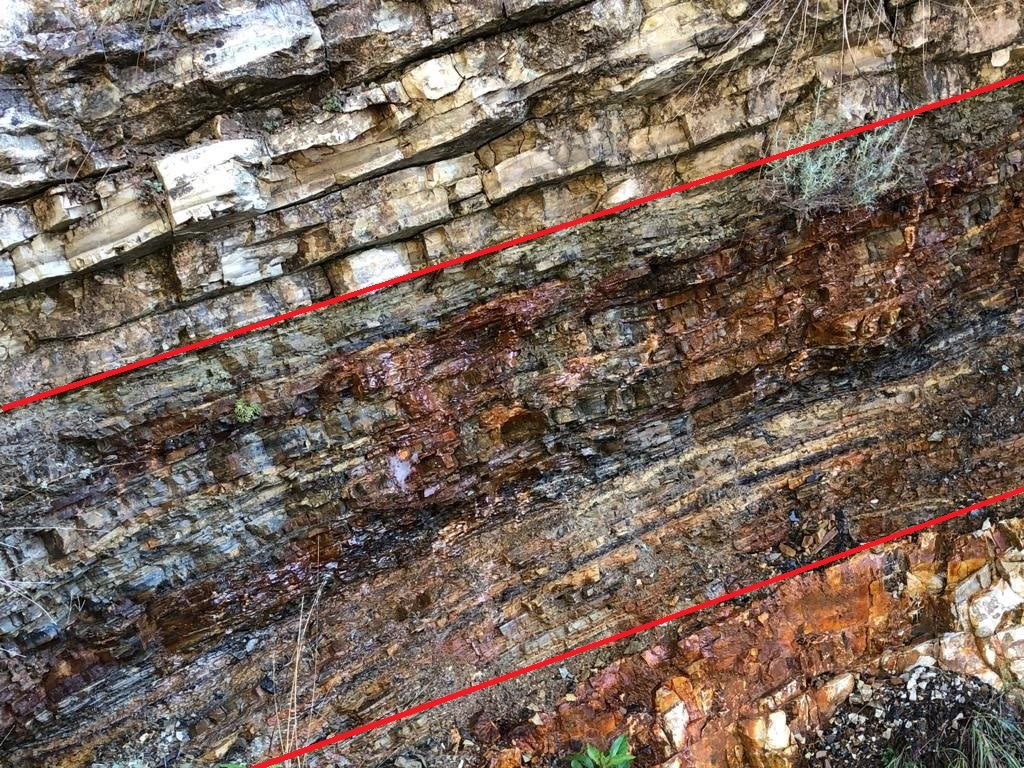
\includegraphics[width=0.66\linewidth]{images/book4/b2-19-bonarelli-level.jpg}
\par\smallskip{\small Lapisan Bonarelli, serpih gelap OAE~2, di antara batu gamping yang pucat; garis-garis
merah, yang digambar oleh fotografernya, menandai alas dan atapnya. (Foto: Picenus, CC~BY-SA~4.0, via
Wikimedia Commons.)}
\end{omfigure}
% ledger: rigo24:oaes

\begin{inthefield}[Mencatat log peristiwa anoksik]
Seorang ahli geologi yang mempelajari sebuah OAE dalam penampang batu gamping pelagis mencatat lognya lapis demi lapis: ketebalan,
warna, laminasi, liang atau ketiadaannya, nodul pirit. Ia mengambil sampel pada selang yang rapat dan teratur
melintasi selang gelap itu dan jauh melampauinya, untuk kandungan karbon organik dan untuk
isotop karbon bahan organik dan karbonat; pergeseran isotop, lebih daripada
warna batuan, yang mengorelasikan peristiwa itu dari satu cekungan ke cekungan berikutnya. Karena serpih
yang paling gelap dapat muncul pada aras yang berbeda di cekungan yang berbeda, kurva isotoplah, bukan serpih
hitamnya, yang diambil sebagai garis waktu.
\end{inthefield}
% ledger: rigo24:oaes, wt24:oae2

\subsection*{Chicxulub}

Akhir Kapur memiliki penyebab dari luar. Volume Tahun~1 menceritakan bagaimana iridium dalam
lempung batas itu mengarah ke suatu tumbukan, dan bagaimana penanggalan argon mengaitkan batas itu dengan kawah Chicxulub.
Struktur itu berdiameter sekitar \qty{200}{km} dan berumur \qty{66}{Ma}; batuan
panasnya memanaskan air yang bersirkulasi selama sedikitnya delapan juta tahun sesudahnya. Model asimetri bawah permukaannya
menunjuk pada penumbuk yang datang dari timur laut dengan sudut 45 sampai \ang{60} terhadap horizontal,
dengan kecepatan tidak kurang daripada kecepatan lepas Bumi, \qty{11.2}{km.s^{-1}}, dan lebih mungkin sekitar
\qty{20}{km.s^{-1}}. Deccan Traps sedang meletus pada waktu yang sama, sebelum dan sesudah
tumbukan; sebuah tinjauan atas bukti-buktinya pada 2010 menyimpulkan bahwa tumbukan itulah yang memicu kepunahan.
% ledger: pickersgill26:chicxulub, collins20:impact, renne:kpg, alvarez:iridium, schulte:kpg, cr03:deccan

\begin{dated}{2026}
Umur-umur dalam bab ini adalah umur pada International Chronostratigraphic Chart versi Juni
2026, sebagaimana digunakan di seluruh seri ini; rekaman muka laut berada pada skala waktu 2012
berkas-berkasnya, dan umur kepunahan adalah umur menurut Kaiho (2022). Bagan itu direvisi ketika penanggalan baru
masuk: periksa versi terbaru sebelum mengutip umur suatu batas.
\end{dated}
% ledger: ics:base.Phanerozoic, data:b4-sealevel, kaiho22:table

\section*{Latihan}\label{sec:b2:phanerozoic-earth:exercises}

Data untuk latihan, kecuali dinyatakan lain: \qty{111.2}{km} per derajat lintang; kedalaman
dasar samudra $d(t) = 2500 + 350\sqrt t$ (\unit{m}, $t$ dalam \unit{Ma}); luas samudra
\qty{362}{\mega km^2}; luas dasar samudra \qty{293}{\mega km^2}; densitas mantel
\qty{3300}{kg.m^{-3}}; air laut \qty{1025}{kg.m^{-3}}; massa atmosfer
\qty{5.1e18}{kg}, massa molar udara dan karbon dioksida \qty{28.97}{g.mol^{-1}} dan
\qty{44.01}{g.mol^{-1}}.
% ledger: earth:Rmean, ps77:depth-age, charette:ocean-volume, data:b4-ridge, katz03:thermo, noaa:seawater-1025, earth:Matm, earth:Mmol, ciaaw:abridged-2024

\begin{exercise}[$\star$]\label{exo:b2:phanerozoic-earth:1}
Dalam model peta-peta itu, Cape Town terletak pada \ang{61.9}~LS \qty{300}{Ma} yang lalu dan New York pada
\ang{3.6}~LS; kini keduanya terletak pada \ang{33.9}~LS dan \ang{40.7}~LU. (a) Manakah dari keempat kota itu yang terletak
dalam jarak \ang{30} dari khatulistiwa \qty{300}{Ma} yang lalu (Paris pada \ang{5.1}~LU, Sydney pada
\ang{59.5}~LS)? (b) Berapa kilometer ke utara Cape Town dan New York masing-masing telah bergeser sejak itu?
(c) Dengan laju rata-rata berapa, dalam sentimeter per tahun?
\end{exercise}
% ledger: data:b4-palaeopos, geonames4:cities

\begin{exercise}[$\star$]\label{exo:b2:phanerozoic-earth:2}
Lima besar terjadi pada 444, 372, 251.9, 201.4, dan \qty{66}{Ma}. (a) Tentukan selang antara
krisis-krisis yang berurutan dan rata-ratanya. (b) Dengan umur rata-rata provinsi beku besar ---
Emeishan 259, Siberia 250, CAMP 201, Karoo--Ferrar 183, Deccan \qty{65.5}{Ma} --- manakah dari
kelima krisis itu yang jatuh dalam \qty{2}{Ma} dari sebuah provinsi? (c) Apakah selang rata-rata membuat krisis-krisis itu periodik?
\end{exercise}
% ledger: kaiho22:table, cr03:table

\begin{exercise}[$\star$]\label{exo:b2:phanerozoic-earth:3}
Kapur Monument Rocks diendapkan dengan laju sekitar \qty{0.036}{mm} per tahun. (a) Berapa lama waktu yang diperlukan untuk
\qty{91}{m} kapur itu? (b) Berapa kali lebih cepat laut naik kini, dengan laju \qty{3.7}{mm} per
tahun? (c) Mengapa dasar laut dapat mengumpulkan hujan sedimen yang begitu lambat tanpa tertimbun oleh lumpur?
\end{exercise}
% ledger: kgs:monument-rocks, ipcc:sea-level-obs

\begin{exercise}[$\star$]\label{exo:b2:phanerozoic-earth:4}
Pada sebuah tebing, dari bawah ke atas: batu pasir sungai dengan akar, pasir pantai dengan cangkang, lumpur
lepas pantai yang kelabu, kapur; lalu kapur itu ditindih lagi oleh pasir pantai. (a) Di mana penampang ini merekam
\omterm{def:b2:phanerozoic-earth:transgression}{transgresi laut}, dan di mana regresi? (b) Apakah transgresi itu membuktikan bahwa muka laut global
naik? (c) Apa yang akan membuatnya lebih meyakinkan?
\end{exercise}

\begin{exercise}[$\star\star$]\label{exo:b2:phanerozoic-earth:5}
Pada kurva jangka panjang Haq dan kawan-kawan, muka laut berada \qty{233}{m} di atas muka laut kini pada
\qty{97}{Ma}. (a) Berapa laju rata-rata penurunannya sejak itu, dalam meter per juta tahun dan dalam
mikrometer per tahun? (b) Bandingkan dengan kenaikan masa kini sebesar \qty{3.7}{mm} per tahun. (c) Kurva New Jersey
yang dikupas balik memberikan sekitar \qty{70}{m} pada waktu yang sama. Mana yang akan kamu percayai untuk
amplitudonya, dan mengapa?
\end{exercise}
% ledger: data:b4-sealevel, ipcc:sea-level-obs, miller05:abstract, miller20:epr

\begin{exercise}[$\star\star$]\label{exo:b2:phanerozoic-earth:6}
Satu denyut CAMP, sekitar \qty{e5}{km^3} basal berdensitas \qty{2900}{kg.m^{-3}},
meletus dalam sekitar 500 tahun. (a) Dengan \qty{0.75}{\percent} karbon dioksida menurut massa, berapa banyak
yang dilepaskannya, dalam kilogram dan dalam mol? (b) Berapa massa karbon dioksida yang dikandung udara pada
\qty{278}{ppm} tahun 1750? (c) Bandingkan. (d) Berapa banyak atmosfer seperti itu yang akan diberikan oleh seluruh provinsi,
\qty{e5}{Gt}?
\end{exercise}
% ledger: capriolo20:camp-co2, ipcc:erf-2xco2, earth:Matm, earth:Mmol, ciaaw:abridged-2024

\begin{exercise}[$\star\star$]\label{exo:b2:phanerozoic-earth:7}
Anggaplah penumbuk Chicxulub sebagai bola berdiameter \qty{10}{km}, berdensitas
\qty{2630}{kg.m^{-3}}. (a) Tentukan massanya. (b) Tentukan energi kinetiknya pada kecepatan terkecil yang mungkin,
\qty{11.2}{km.s^{-1}}, dan pada \qty{20}{km.s^{-1}}. (c) Bumi kehilangan \qty{47}{TW} kalor
internal melalui permukaannya. Berapa tahun kehilangan itu yang diwakili oleh masing-masing energi?
\end{exercise}
% ledger: alvarez:iridium, collins20:impact, b2dd10:half-space

\begin{exercise}[$\star\star$]\label{exo:b2:phanerozoic-earth:8}
(a) Sebutkan ciri-ciri yang membuat serpih hitam merekam suatu \omterm{def:b2:phanerozoic-earth:oae}{peristiwa anoksik samudra}. (b) Pasangkan setiap
peristiwa dengan sebuah provinsi yang umurnya hampir sama: Toarsium awal, \qty{183}{Ma}; OAE~1a,
\qty{120}{Ma}; diketahui Karoo--Ferrar pada \qty{183}{Ma} dan Ontong Java pada \qty{122}{Ma}. (c) Mengapa
kebetulan umur yang sama tidak cukup untuk membuktikan bahwa sebuah provinsi menyebabkan suatu peristiwa?
\end{exercise}
% ledger: rigo24:oaes, cr03:table

\begin{exercise}[$\star\star$]\label{exo:b2:phanerozoic-earth:9}
Dalam model itu, Paris terletak pada \ang{60.9}~LS \qty{500}{Ma} yang lalu dan pada \ang{5.1}~LU \qty{300}{Ma} yang lalu.
(a) Tentukan pergeserannya ke utara dalam derajat dan dalam kilometer, dan laju rata-ratanya dalam
sentimeter per tahun. (b) Bandingkan dengan laju sejak \qty{300}{Ma}
(\cref{ex:b2:phanerozoic-earth:paris}). (c) Mengapa laju itu merupakan nilai minimum?
\end{exercise}
% ledger: data:b4-palaeopos

\begin{exercise}[$\star\star\star$]\label{exo:b2:phanerozoic-earth:10}
Misalkan sebaliknya luas dasar samudra berkurang secara linear terhadap umur, dari maksimum pada umur 0 sampai nol
pada umur $T$. (a) Tunjukkan bahwa umur rata-ratanya $T/3$ dan rata-rata $\sqrt t$ adalah
$\tfrac{8}{15}\sqrt T$. (b) Dengan umur rata-rata \qty{64.2}{Ma}, tentukan $T$ dan kedalaman rata-ratanya. (c)
Tentukan penurunan kedalaman rata-rata ketika laju pemekaran berlipat dua, dan bandingkan dengan
\qty{774}{m} dari model merata. (d) Tunjukkan bahwa dalam kedua model penurunan itu mendekati $0.93\,c\sqrt{\bar
t}\,(1 - f^{-1/2})$, dengan $\bar t$ umur rata-rata.
\end{exercise}

\begin{exercise}[$\star\star\star$]\label{exo:b2:phanerozoic-earth:11}
(a) Dari \cref{prop:b2:phanerozoic-earth:ridge}, tunjukkan bahwa $\Delta s(f) = \Delta s(2)\,(1 -
f^{-1/2})/(1 - 2^{-1/2})$. (b) Dengan $\Delta s(2) = \qty{432}{m}$, tentukan rentang $f$ yang
memberikan puncak Kapur, 50 sampai \qty{150}{m}. (c) Apa yang akan terjadi jika laju pemekaran melambat menjadi 0.8 kali
laju kini? (d) Mengapa muka laut jangka panjang yang ditentukan oleh punggungan merupakan sinyal yang lambat, berapa pun perubahan
lajunya?
\end{exercise}
% ledger: data:b4-ridge, miller05:abstract

\begin{exercise}[$\star\star\star$]\label{exo:b2:phanerozoic-earth:12}
Misalkan spesies punah dengan laju tetap, sehingga fraksi suatu kohort yang bertahan selama waktu
$t$ adalah $2^{-t/m}$, dengan median umur spesies $m = \qty{2}{Ma}$. (a) Berapa fraksi
kohort yang hilang setelah \qty{7.4}{Ma}, panjang rata-rata jenjang dalam analisis 1982? (b) Berapa lama
kepunahan latar akan melenyapkan \qty{81}{\percent} spesies? (c) Krisis akhir Perm
berlangsung sekitar \qty{60}{ka}. Berapa kali lebih cepat krisis itu? (d) Mengapa resolusi waktu yang kasar
mengaburkan perbedaan antara kepunahan massal dan kepunahan latar?
\end{exercise}
% ledger: marshall23:resolution, stanley16:permian, burgess:end-permian

\begin{problem}[{Soal akhir pekan --- Ketika punggungan memekar cepat}]\label{pb:b2:phanerozoic-earth:1}
Soal ini menanyakan seberapa tinggi laut akan naik, dan seberapa luas daratan yang akan ditenggelamkannya, jika
punggungan memekar dua kali lebih cepat. Gunakan data latihan; umur rata-rata dasar samudra adalah
\qty{64.2}{Ma}, punggungan seluruhnya sepanjang \qty{65000}{km}, samudra masa kini menampung
\qty{1.33e9}{km^3}, dan daratan menutupi \qty{148}{\mega km^2}. Tabel memberikan persen daratan
masa kini yang terletak kurang dari $h$ di atas muka laut, dari kisi ETOPO1 satu derajat.
\begin{center}
\small
\begin{tabular}{lcccccc}
\hline
$h$ (\unit{m}) & 0 & 100 & 200 & 300 & 400 & 500 \\
daratan di bawah $h$ (\unit{\percent}) & 0 & 14.9 & 28.2 & 38.7 & 48.1 & 55.8 \\
\hline
\end{tabular}
\end{center}
Anggaplah, seperti dalam \cref{prop:b2:phanerozoic-earth:ridge}, bahwa setiap umur dasar samudra antara 0 dan
umur $\tau$ saat dasar samudra itu tersubduksi menempati luas yang sama.

\noindent\textbf{Bagian I --- Dasar samudra masa kini.}
\begin{enumerate}
  \item Tentukan kedalaman dasar samudra pada umur 0, 25, 64.2, dan \qty{100}{Ma}.
  \item Tentukan $\tau$ dari umur rata-rata, dan kedalaman dasar samudra tertua.
  \item Tentukan laju pemekaran penuh rata-rata $u = A_{\text{f}}/(L\tau)$, dalam kilometer per juta
        tahun dan dalam milimeter per tahun. Apakah itu laju lambat, menengah, atau cepat?
  \item Tunjukkan bahwa kedalaman rata-rata dasar samudra adalah $2500 + \tfrac23 \times 350\sqrt\tau$, dan
        hitunglah.
  \item Kedalaman rata-rata terukur dasar samudra yang telah ditentukan umurnya adalah \qty{4265}{m}. Berikan dua alasan mengapa
        model itu lebih dalam.
  \item Berapa volume air yang akan berada di atas dasar samudra dalam model itu? Bandingkan dengan volume
        seluruh samudra.
\end{enumerate}

\noindent\textbf{Bagian II --- Punggungan dalam penampang.}
\begin{enumerate}[resume]
  \item Tentukan laju pemekaran setengah $v$, sampai \qty{0.1}{km.Ma^{-1}} terdekat, dan lebar
        dasar samudra di setiap sisi punggungan.
  \item Berapa kedalaman dasar samudra pada jarak \qty{1000}{km} dari sumbu?
  \item Tunjukkan bahwa penampang punggungan di atas kedalaman dasar samudra tertua, dengan menghitung
        kedua sayapnya, memiliki luas $\tfrac23 v c\,\tau^{3/2}$, dan hitunglah dalam
        kilometer persegi.
  \item Tentukan volume seluruh sistem punggungan di atas kedalaman itu.
  \item Berapa fraksi volume samudra yang diwakilinya?
  \item Mengapa punggungan yang memekar lebih cepat rata-rata berdiri lebih tinggi?
\end{enumerate}

\noindent\textbf{Bagian III --- Dua kali lebih cepat.}
\begin{enumerate}[resume]
  \item Laju pemekaran berlipat dua dengan luas dasar samudra dan panjang punggungan yang sama. Tentukan $\tau$ yang baru
        dan kedalaman rata-rata yang baru.
  \item Berapa besar penurunan kedalaman rata-ratanya?
  \item Berapa volume air yang didorong keluar dari cekungan oleh dasar samudra?
  \item Jika disebarkan di atas samudra masa kini, berapa tinggi air itu akan menaikkan laut?
  \item Masukkan penurunan dasar samudra di bawah air tambahan untuk menentukan kenaikan $\Delta s$.
  \item Puncak Kapur jangka panjang sekitar \qty{100}{m}. Kenaikan laju pemekaran berapa
        yang akan memberikan nilai itu?
\end{enumerate}

\noindent\textbf{Bagian IV --- Laut di atas daratan.}
\begin{enumerate}[resume]
  \item Berapa luas daratan yang akan dibanjiri oleh kenaikan \qty{100}{m}?
  \item Berapa luas yang akan dibanjiri oleh kenaikan \qty{432}{m}, dengan interpolasi dalam tabel?
  \item Mengapa laut harus naik kurang dari \qty{432}{m} begitu laut itu menyebar di atas daratan?
  \item Tentukan volume yang diperlukan untuk menaikkan laut dalam langkah-langkah \qty{100}{m} sampai \qty{400}{m},
        dengan merata-ratakan luas yang tergenang selama setiap langkah (\cref{prop:b2:phanerozoic-earth:flooding}).
        Volume yang harus ditempatkan adalah $\qty{0.432}{km} \times \qty{362}{\mega km^2}$. Di mana
        laut berhenti?
  \item Berapa persen daratan masa kini yang kemudian ditutupinya?
  \item Sebagai ringkasan: dalam model ini, berapa tinggi laut akan naik jika laju pemekaran berlipat dua?
\end{enumerate}
\end{problem}
% ledger: ps77:depth-age, seton:mean-age, seton:rate-classes, noaa:ridge, charette:ocean-volume, data:b4-ridge, data:b4-floor-depth, katz03:thermo, noaa:seawater-1025, data:b4-hyps, miller05:abstract
